\PassOptionsToPackage{table}{xcolor}

\documentclass[
%	handout,
	notes=none,
	aspectratio=169
]{beamer}

% Comment out the following line to hide the notes
%\setbeameroption{show notes}

\input{macros}

\mode<handout>{%
	\pgfpagesuselayout{8 on 1}[a4paper,border shrink=5mm]
	\setbeameroption{show notes}
}

\usefolder{theme}
\usetheme{TuringDark}
\graphicspath{{./graphics/}}

\begin{document}

\title{Porting the Aurora Weather Model to Intel Accelerated Hardware}
\subtitle{}
\author{Iain Stenson, Rosie Wood, David Llewellyn-Jones, Tomas Lazauskas}
\date{15 May 2026}
\def\cornerimagefilename{aurora-title.jpg}

%%%%%%%%%%%%%%%%%%%%%%%%%%%%%%%%%%%%%%%%%

\renewcommand{\thefootnote}{\arabic{footnote}}

\frame{
\titlepage
}
\note{
}

\renewcommand{\thefootnote}{\fnsymbol{footnote}}

%%%%%%%%%%%%%%%%%%%%%%%%%%%%%%%%%%%%%%%%%

\begin{frame}
\frametitle{Aurora: A Foundation Model for the Earth}

\begin{columns}[T]
\begin{column}[T]{0.6\textwidth}
\setlength{\parskip}{0.5em}

\vspace{0.0cm}
\begin{enumerate}
\setlength{\parskip}{0.5em}
\item Predicts atmospheric variables
\item Adapts to specialised forecasting tasks
\item Microsoft Cambridge
\end{enumerate}

\end{column}
\begin{column}[T]{0.35\textwidth}
\setlength{\parskip}{0.5em}

\vspace{0.0cm}
\begin{enumerate}
\setlength{\parskip}{0.5em}
\item Ease of porting
\item Similarity of results
\item Speed
\end{enumerate}

\end{column}
\end{columns}

\end{frame}
\note{
}

%%%%%%%%%%%%%%%%%%%%%%%%%%%%%%%%%%%%%%%%%

{
\definecolor{slidebg}{rgb}{1.0,1.0,1.0}
\begin{frame}
\frametitle{}

\begin{columns}[T]
\begin{column}[T]{0.59\textwidth}

\vspace{-0.2cm}
\hspace{0.0cm}

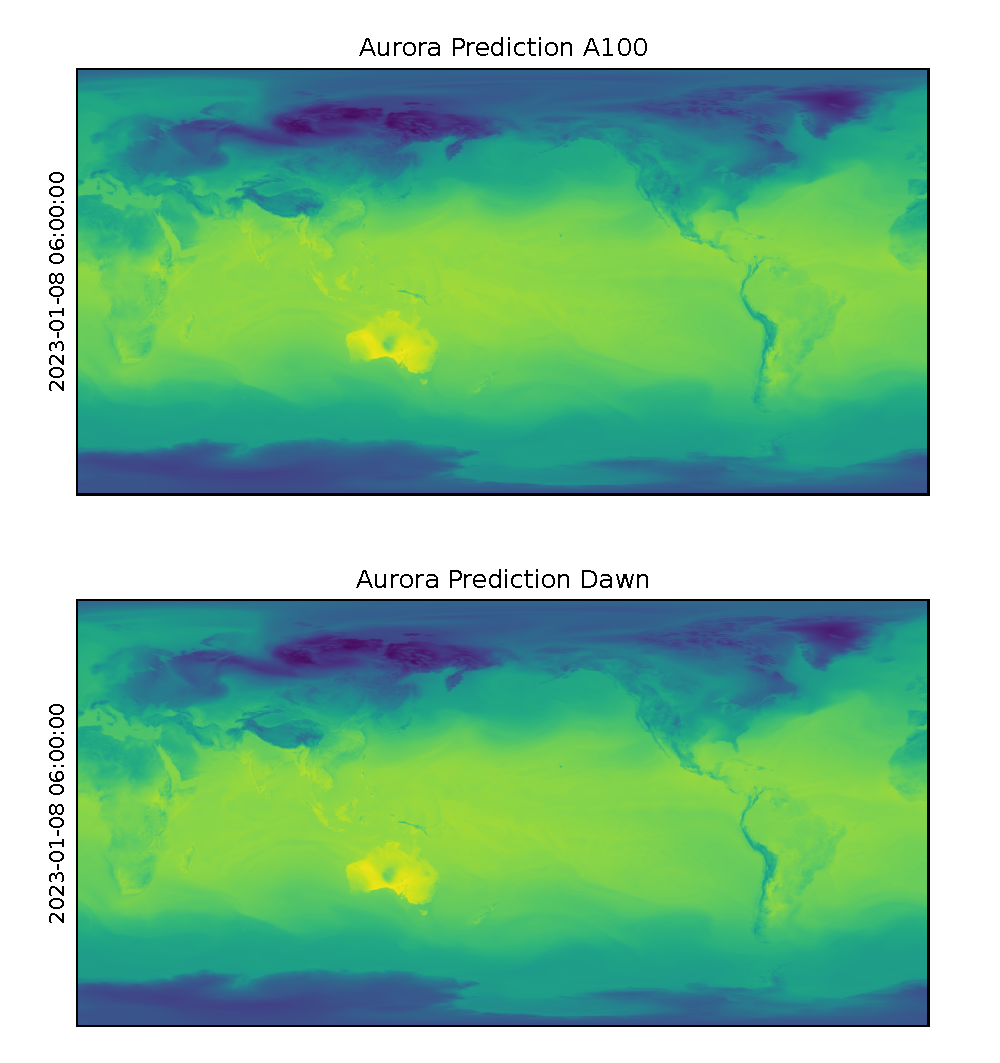
\includegraphics[width=1.0\textwidth]{plot-pvg}

\end{column}
\end{columns}

\end{frame}
\note{
\begin{enumerate}
\item Rollout
\end{enumerate}
}
}

%%%%%%%%%%%%%%%%%%%%%%%%%%%%%%%%%%%%%%%%%

{
\definecolor{slidebg}{rgb}{1.0,1.0,1.0}
\begin{frame}
\frametitle{}

\begin{columns}[T]
\begin{column}[T]{1.0\textwidth}

\vspace{-0.2cm}
\hspace{0.0cm}

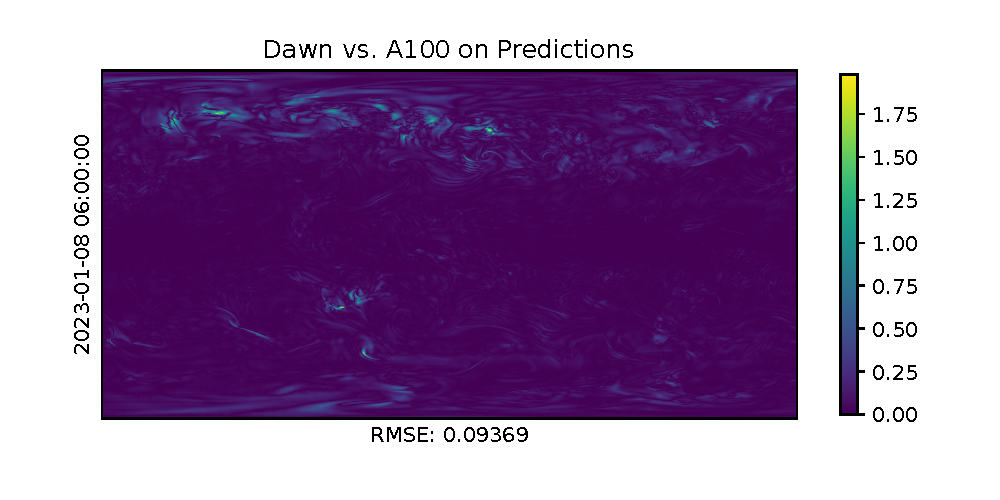
\includegraphics[width=1.0\textwidth]{plot-errors-dawn-bask}

\end{column}
\end{columns}

\end{frame}
\note{
\begin{enumerate}
\item Rollout
\end{enumerate}
}
}

%%%%%%%%%%%%%%%%%%%%%%%%%%%%%%%%%%%%%%%%%

{
\definecolor{slidebg}{rgb}{1.0,1.0,1.0}
\begin{frame}
\frametitle{}

\begin{columns}[T]
\begin{column}[T]{0.85\textwidth}

\vspace{0.2cm}
\hspace{0.0cm}

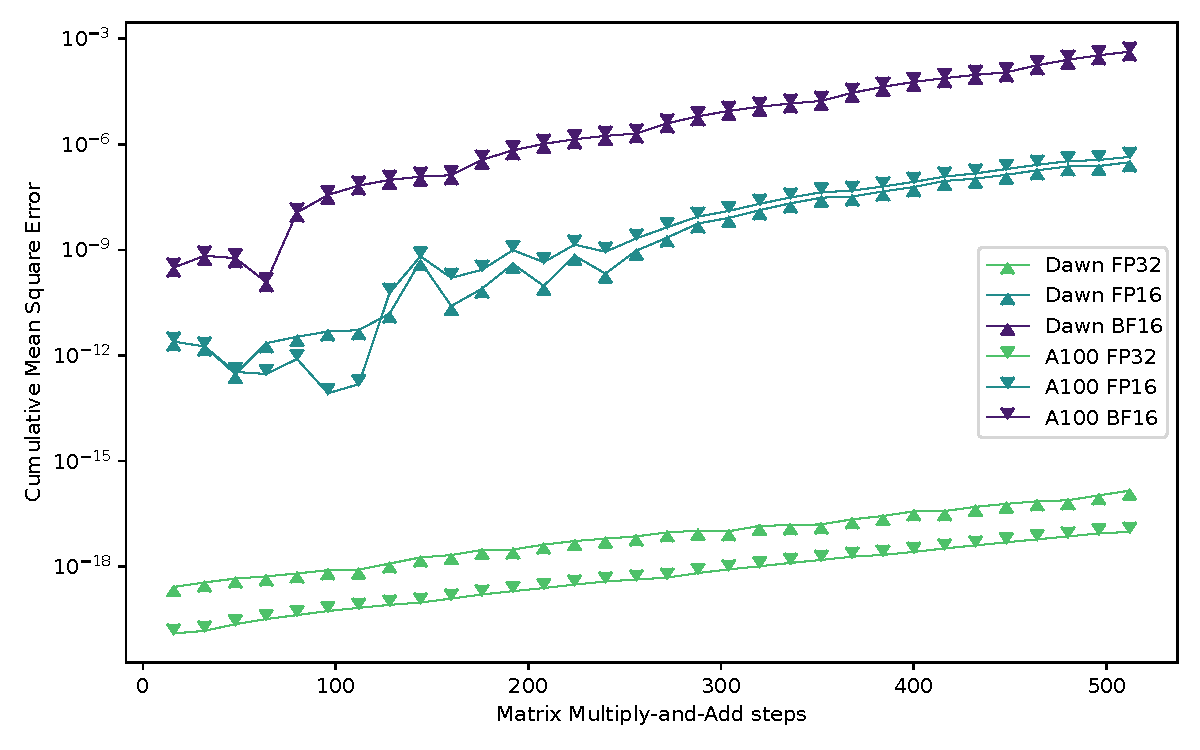
\includegraphics[width=1.0\textwidth]{plot-error-dev-mad-1024x1024-s42}

\end{column}
\end{columns}

\end{frame}
\note{
\begin{enumerate}
\item Rollout
\end{enumerate}
}
}

%%%%%%%%%%%%%%%%%%%%%%%%%%%%%%%%%%%%%%%%%

{
\definecolor{slidebg}{rgb}{1.0,1.0,1.0}
\begin{frame}
<presentation:0>[noframenumbering]
\frametitle{}

\begin{columns}[T]
\begin{column}[T]{0.85\textwidth}

\vspace{0.2cm}
\hspace{0.0cm}

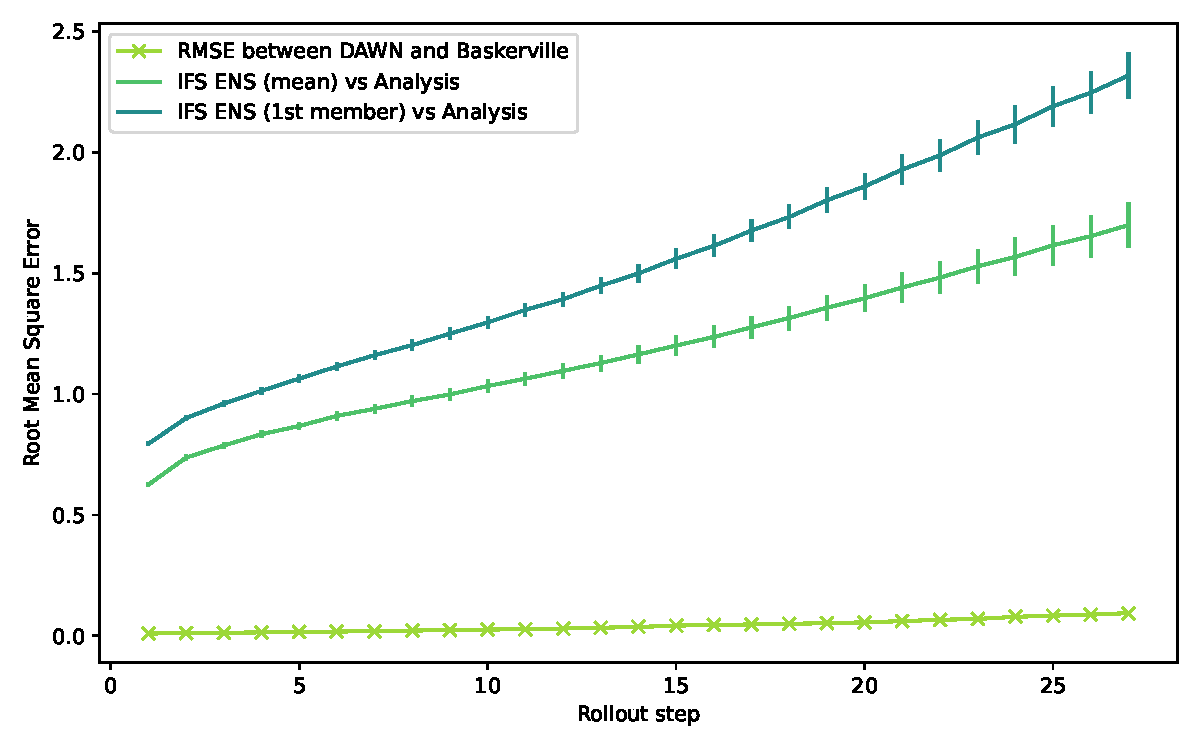
\includegraphics[width=1.0\textwidth]{plot-weatherbench-comparison}

\end{column}
\end{columns}

\end{frame}
\note{
\begin{enumerate}
\item Rollout
\end{enumerate}
}
}

%%%%%%%%%%%%%%%%%%%%%%%%%%%%%%%%%%%%%%%%%

\begin{frame}
<presentation:0>[noframenumbering]
\frametitle{Inference timing}

\begin{columns}[T]
\begin{column}[T]{1.0\textwidth}

\vspace{-0.2cm}
\hspace{0.0cm}

\begin{table}[t]
    \small
    \setlength\extrarowheight{0.8em}
    \centering
    \hbadness=99999
    \begin{tabular}{ll|rrrr}
        \parbox{1cm}{System \\} & \parbox{0.8cm}{Hierarchy \\} & \parbox{2.0cm}{\raggedleft Mean time-step /s} &  \parbox{1.8 cm}{\raggedleft Time for first step /s} & \parbox{1.8cm}{\raggedleft Time for 28 steps /s} & \parbox{1.5cm}{\raggedleft Total run \\ time /s} \\ \hline
        Dawn & \textit{flat} & 6.21 &  17.56&185.29& 248.45\\
        Dawn & \textit{composite} & 6.72 &  18.37&199.70& 262.76\\
        A100 & N/A& 6.09 & 15.86 & 180.54 & 255.48\\
    \end{tabular}
\end{table}

\end{column}
\end{columns}

\end{frame}
\note{
\begin{enumerate}
\item Rollout
\end{enumerate}
}

%%%%%%%%%%%%%%%%%%%%%%%%%%%%%%%%%%%%%%%%%

\begin{frame}
<presentation:0>[noframenumbering]
\frametitle{Inference timing}

\begin{columns}[T]
\begin{column}[T]{1.0\textwidth}

\vspace{-0.2cm}
\hspace{0.0cm}

\begin{table}[t]
    \small
    \setlength\extrarowheight{0.8em}
    \centering
    \hbadness=99999
    \begin{tabular}{ll|rrrr}
        \parbox{1cm}{System \\} & \parbox{0.8cm}{Hierarchy \\} & \parbox{2.0cm}{\raggedleft Mean time-step /s} &  \parbox{1.8 cm}{\raggedleft Time for first step /s} & \parbox{1.8cm}{\raggedleft Time for 28 steps /s} & \parbox{1.5cm}{\raggedleft Total run \\ time /s} \\ \hline
        Dawn & \textit{flat} & \circletext{6.21} & 17.56&185.29 & 248.45\\
        Dawn & \textit{composite} & \circletext{6.72} & 18.37 & 199.70 & 262.76\\
        A100 & N/A & \circletext{6.09} & 15.86 & 180.54 & 255.48\\
    \end{tabular}
\end{table}

\end{column}
\end{columns}

\end{frame}
\note{
\begin{enumerate}
\item Rollout
\end{enumerate}
}
%%%%%%%%%%%%%%%%%%%%%%%%%%%%%%%%%%%%%%%%%

\begin{frame}
\frametitle{}

\begin{columns}[T]
\begin{column}[T]{0.75\textwidth}

\vspace{0.2cm}
\hspace{0.0cm}

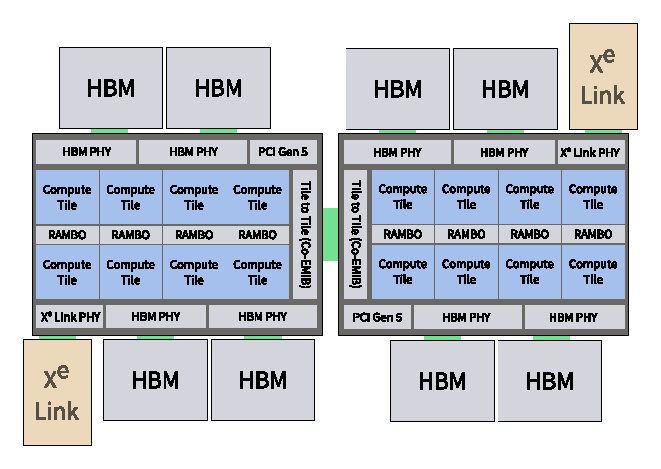
\includegraphics[width=1.0\textwidth]{ponteveccio}

\end{column}
\end{columns}

\end{frame}
\note{
\begin{enumerate}
\item Rollout
\end{enumerate}
}

%%%%%%%%%%%%%%%%%%%%%%%%%%%%%%%%%%%%%%%%%

\begin{frame}
\frametitle{Fine-tuning Timings}

\begin{columns}[T]
\begin{column}[T]{1.0\textwidth}

\vspace{-0.2cm}
\hspace{0.0cm}

\begin{table}[t]
    \small
    \setlength\extrarowheight{0.4em}
    \centering
    \hbadness=99999
    \begin{tabular}{rrr|rrr}
          \parbox{1cm}{GPUs \\} & \parbox{1cm}{Devices \\} & \parbox{1.5cm}{\raggedleft Hierarchy \\ \hfill} & \parbox{3.0cm}{\raggedleft Compute time per iteration /s} & \parbox{3.0cm}{\raggedleft Wall-clock time per iteration /s} & \parbox{2.0cm}{\raggedleft Total run time /s} \\ \hline
          1 & 1 & \textit{flat} & 6.86 & 6.86 & 257.43 \\
          1 & 2 & \textit{flat} & 7.84 & 3.92 & 176.54 \\
          4 & 4 & \textit{flat} & 8.13 & 2.03 & 122.72 \\
          4 & 8 & \textit{flat} & 7.73 & 0.97 & 90.99 \\
          1 & 1 & \textit{composite} & 11.10 & 11.10 & 391.70 \\
          2 & 2 & \textit{composite} & 11.45 & 5.72 & 259.46 \\
          4 & 4 & \textit{composite} & 11.54 & 2.89 & 152.56 \\
          1 & 1 & A100 & 3.20 & 3.20 & 145.53 \\
          2 & 2 & A100 & 3.25 & 1.62 & 104.85 \\
          4 & 4 & A100 & 3.29 & 0.82 & 81.72 \\
    \end{tabular}
\end{table}

\end{column}
\end{columns}

\end{frame}
\note{
\begin{enumerate}
\item Rollout
\end{enumerate}
}

%%%%%%%%%%%%%%%%%%%%%%%%%%%%%%%%%%%%%%%%%

\begin{frame}
\frametitle{Fine-tuning Timings}

\begin{columns}[T]
\begin{column}[T]{1.0\textwidth}

\vspace{-0.2cm}
\hspace{0.0cm}

\begin{table}[t]
    \small
    \setlength\extrarowheight{0.4em}
    \centering
    \hbadness=99999
    \begin{tabular}{rrr|rrr}
          \parbox{1cm}{GPUs \\} & \parbox{1cm}{Devices \\} & \parbox{1.5cm}{\raggedleft Hierarchy \\ \hfill} & \parbox{3.0cm}{\raggedleft Compute time per iteration /s} & \parbox{3.0cm}{\raggedleft Wall-clock time per iteration /s} & \parbox{2.0cm}{\raggedleft Total run time /s} \\ \hline
          1 & 1 & \textit{flat} & \circletext{6.86} & 6.86 & 257.43 \\
          1 & 2 & \textit{flat} & 7.84 & 3.92 & 176.54 \\
          4 & 4 & \textit{flat} & 8.13 & 2.03 & 122.72 \\
          4 & 8 & \textit{flat} & 7.73 & 0.97 & 90.99 \\ \hdashline
          1 & 1 & \textit{composite} & \circletext{11.10} & 11.10 & 391.70 \\
          2 & 2 & \textit{composite} & 11.45 & 5.72 & 259.46 \\
          4 & 4 & \textit{composite} & 11.54 & 2.89 & 152.56 \\ \hdashline
          1 & 1 & A100 & \circletext{3.20} & 3.20 & 145.53 \\
          2 & 2 & A100 & 3.25 & 1.62 & 104.85 \\
          4 & 4 & A100 & 3.29 & 0.82 & 81.72 \\
    \end{tabular}
\end{table}

\end{column}
\end{columns}

\end{frame}
\note{
\begin{enumerate}
\item Rollout
\end{enumerate}
}

%%%%%%%%%%%%%%%%%%%%%%%%%%%%%%%%%%%%%%%%%

\begin{frame}
\frametitle{Fine-tuning Timings}

\begin{columns}[T]
\begin{column}[T]{1.0\textwidth}

\vspace{-0.2cm}
\hspace{0.0cm}

\begin{table}[t]
    \small
    \setlength\extrarowheight{0.4em}
    \centering
    \hbadness=99999
    \begin{tabular}{rrr|rrr}
          \parbox{1cm}{GPUs \\} & \parbox{1cm}{Devices \\} & \parbox{1.5cm}{\raggedleft Hierarchy \\ \hfill} & \parbox{3.0cm}{\raggedleft Compute time per iteration /s} & \parbox{3.0cm}{\raggedleft Wall-clock time per iteration /s} & \parbox{2.0cm}{\raggedleft Total run time /s} \\ \hline
          1 & 1 & \textit{flat} & 6.86 & 6.86 & 257.43 \\
          1 & 2 & \textit{flat} & 7.84 & \circletext{3.92} & 176.54 \\
          4 & 4 & \textit{flat} & 8.13 & 2.03 & 122.72 \\
          4 & 8 & \textit{flat} & 7.73 & 0.97 & 90.99 \\ \hdashline
          1 & 1 & \textit{composite} & 11.10 & 11.10 & 391.70 \\
          2 & 2 & \textit{composite} & 11.45 & 5.72 & 259.46 \\
          4 & 4 & \textit{composite} & 11.54 & 2.89 & 152.56 \\ \hdashline
          1 & 1 & A100 & 3.20 & \circletext{3.20} & 145.53 \\
          2 & 2 & A100 & 3.25 & 1.62 & 104.85 \\
          4 & 4 & A100 & 3.29 & 0.82 & 81.72 \\
    \end{tabular}
\end{table}

\end{column}
\end{columns}

\end{frame}
\note{
\begin{enumerate}
\item Rollout
\end{enumerate}
}

%%%%%%%%%%%%%%%%%%%%%%%%%%%%%%%%%%%%%%%%%

{
\definecolor{slidebg}{rgb}{1.0,1.0,1.0}
\begin{frame}
\frametitle{}

\begin{columns}[T]
\begin{column}[T]{0.7\textwidth}

\vspace{0.2cm}
\hspace{0.0cm}

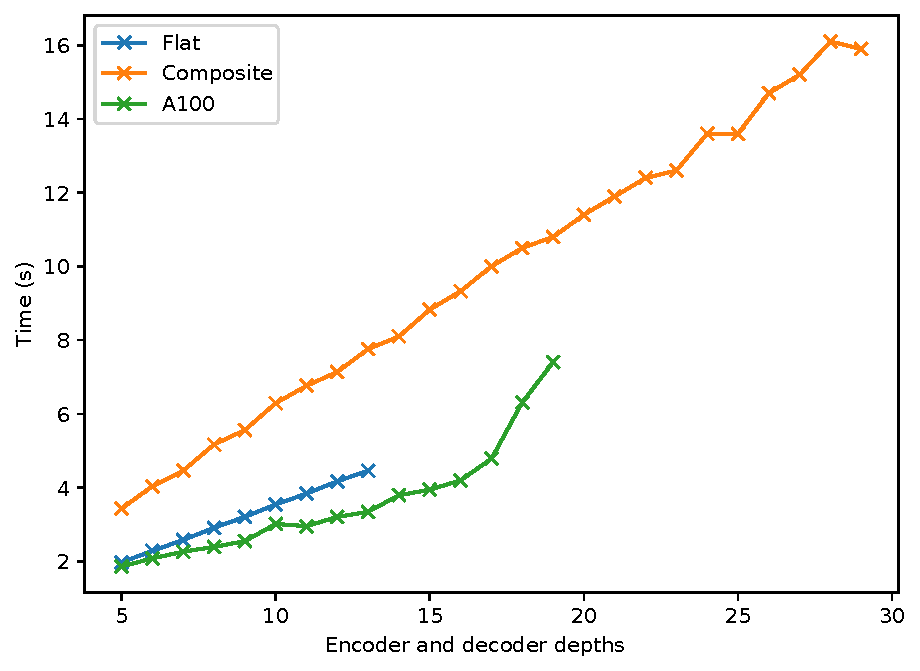
\includegraphics[width=1.0\textwidth]{flat-vs-composite}

\end{column}
\end{columns}

\end{frame}
\note{
\begin{enumerate}
\item Rollout
\end{enumerate}
}
}

%%%%%%%%%%%%%%%%%%%%%%%%%%%%%%%%%%%%%%%%%

\begin{frame}[fragile]
\frametitle{Links}

\begin{columns}[T]
\begin{column}[T]{1.0\textwidth}
\setlength{\leftmargini}{8.5em}
\vspace{0.0cm}

\begin{itemize}
\setlength{\parskip}{1.5em}
\item[Aurora \quad] \href{https://github.com/microsoft/aurora/}{\path{https://github.com/microsoft/aurora/} \\ \path{}}


\item[Report \quad] \href{https://github.com/alan-turing-institute/aurora-hpc}{\path{https://github.com/alan-turing-institute/} \\ \path{aurora-hpc}}

\item[Slides \quad] \href{https://github.com/alan-turing-institute/airr-at-cam-2026-aurora}{\path{https://github.com/alan-turing-institute/} \\ \path{airr-at-cam-2026-aurora}}

\end{itemize}

\vspace{2.0em}

\centering

With thanks to the Dawn and Baskerville teams.\qquad \qquad \qquad

\end{column}
\end{columns}

\end{frame}
\note{
\fontsize{7pt}{8pt}{\bibliographystyle{ieeetr}}
\bibliography{slides}
}

%%%%%%%%%%%%%%%%%%%%%%%%%%%%%%%%%%%%%%%%%

\end{document}
